\section{Results}
In this section, the performance of the various document knowledge transfer approaches in the LCR-Rot-hop++ model is analysed. First, the accuracy of each model is analysed, before we examine the confusion matrix of the best performing model compared to the benchmark, to consider the performance per sentiment. Last, in a sensitivity analysis it is shown how the performance is affected by changes in $\lambda$. The  hyperparameters for each of the models can be found in Table \ref{tab:hyperparams} in the appendix.

%In the following subsection, the results of several sensitivity analyses are presented, to show how the performance is affected by changes in $\lambda$ and in the size of the pretraining corpora. The  hyperparameters for each of the models can be found in Table \ref{tab:hyperparams} in the appendix.

\subsection{Model Performance}

Table \ref{tab:resultsModel} shows the results of the benchmark LCR-Rot-hop++ model with different hyperparameters and different combinations of document knowledge transfer approaches, for the data of SemEval 2015 and SemEval 2016. All losses, including that of the benchmark LCR-Rot-hop++ model without document knowledge transfer, are regularised using the L1 and L2 regularisation terms, allowing for a fair comparison. We find that several TL models outperform the benchmark LCR-Rot-hop++ model, for both datasets, suggesting there is added value in incorporating document knowledge transfer in the base model.

\begin{table}[h]
\caption{Results of LCR-Rot-hop++ with various forms of document knowledge transfer, alongside the benchmark model without document knowledge transfer, for the SemEval 2015 and SemEval 2016 datasets.}
\label{tab:resultsModel}
\setlength{\tabcolsep}{38pt}
\begin{tabular}{@{}lcc@{}}
\toprule
\multicolumn{1}{c}{\multirow{2}{*}{Settings}} & \multicolumn{2}{c}{Accuracy} \\ \cmidrule(l){2-3} 
\multicolumn{1}{c}{}                          & SemEval 2015  & SemEval 2016 \\ \midrule
\textit{Benchmark model}                      &               &              \\
LCR-Rot-hop++                                 & 79.5\%        & 88.1\%       \\ \midrule
\textit{FT-based models}                      &               &              \\
MULT+FT                                       & 79.7\%        & 88.3\%       \\
PRET+FT                                       & 80.5\%        & 88.6\%       \\
PRET+MULT+FT                                  & 79.8\%         & 88.4\%       \\ \midrule
\textit{MULT-based models}                    &               &              \\
MULT                                          & 81.7\%        & 88.5\%       \\
MULT+FT                                       & 79.2\%        & 88.4\%       \\
PRET+MULT                                     & 81.2\%        & 88.2\%       \\
PRET+MULT+FT                                  & 81.3\%        & 88.2\%       \\ \bottomrule
\end{tabular}
\footnotesize\textit{Note}. The FT-based models are constructed using the optimal hyperparameters from a model with only the FT stage, as is the LCR-Rot-hop++ benchmark model. The MULT-based models use the optimal hyperparameters for a pure MULT model.
\vspace{-3mm}
\end{table}
For the SemEval 2015 dataset, all models with TL outperform the benchmark model, with the exception of the MULT-based MULT+FT. The largest improvement in accuracy, 2.2 percentage points, is observed for the MULT model. Similarly, for the SemEval 2016 dataset, we observe that all TL models outperform the benchmark. Here, the biggest improvements are observed for the PRET+FT and MULT models, which exceed the accuracy of the benchmark model by 0.5 and 0.4 percentage points, respectively. The differences in performance for this dataset are smaller, likely because it is larger and more balanced. Given that transfer learning aims to handle limited data availability and data imbalance by supplying the model with additional examples of a similar task, it is indeed to be expected that these approaches have greater impact in the 2015 dataset. 

Based on the accuracy measures, we conclude that the analysed TL models show potential to boost the accuracy of the existing LCR-Rot-hop++ model. Overall, the MULT model performs best, as it leads to the greatest improvements in accuracy across the two datasets. In comparison to the existing state-of-the-art HAABSA++ model, we observe that our MULT model outperforms HAABSA++ for the SemEval 2016 dataset, by 1.5 percentage points, and matches its performance for the SemEval 2015 dataset, at 81.7\% accuracy. 

One plausible reason for MULT outperforming PRET approaches is catastrophic forgetting \cite{Chen2020}. Knowledge learned in the PRET stage might be forgotten when the model is retrained on the main task. In MULT, the main and auxiliary task are learned simultaneously, making the document knowledge more recent and prevalent. As shown in \cite{Chen2020}, multi-task learning provides a solution to catastrophic forgetting.

%We note that the HAABSA++ model does not include the L1 and L2 regularisation terms, so we cannot entirely attribute the increased performance for the 2016 data to our TL approach, and there might also have been slight computational differences, for example with the searched range for hyperparameter tuning, which could explain the differences in the results. Still, we conclude that our model demonstrates comparable performance to HAABSA++ across the two basic datasets. 

\subsection{Model Performance per Sentiment Class}
Next, we compare the confusion matrices of the LCR-Rot-hop++ benchmark model and the MULT model. This comparison allows us to further investigate how the classifications differ per sentiment. The SemEval 2015 data will be used as this is where the greatest differences are expected, as explained in the previous section. We also consider the confusion matrix for the PRET+FT model, as it showed a slight improvement over the MULT model for the SemEval 2016 dataset. As the confusion matrices for the MULT and PRET+FT models show similar results, the PRET+FT confusion matrix is displayed in Table \ref{tab:confusion matrix:pret} in the appendix. 
\begin{table}[h]
\caption{Confusion matrix of the benchmark LCR-Rot-hop++ model for the SemEval 2015 data.}
\label{tab:confusion matrix LCR}
\setlength{\tabcolsep}{28.3pt}
\begin{tabular}{@{}lccc@{}}
\toprule
                   & \multicolumn{3}{c}{Predicted sentiment} \\ \midrule
Observed sentiment & Negative     & Neutral    & Positive    \\ \midrule
Negative           & 179          & 0          & 29          \\
Neutral            & 20           & 0          & 18          \\
Positive           & 56           & 0          & 298         \\ \bottomrule
\end{tabular}
%\vspace{-5mm}
\end{table}

\vspace{-3mm}

\begin{table}[h]
\caption{Confusion matrix of the MULT model with document knowledge transfer for the SemEval 2015 data.}
\label{tab:confusion matrix:mult}
\setlength{\tabcolsep}{28.3pt}
\begin{tabular}{@{}lccc@{}}
\toprule
                   & \multicolumn{3}{c}{Predicted sentiment} \\ \midrule
Observed sentiment & Negative     & Neutral    & Positive    \\ \midrule
Negative           & 157          & 4          & 47          \\
Neutral            & 4           & 2          & 23          \\
Positive           & 21           & 2          & 331         \\ \bottomrule
\end{tabular}
\end{table}

Table \ref{tab:confusion matrix LCR} shows that the LCR-Rot-hop++ model never predicts a neutral sentiment. This is likely caused by the sparsity of neutral observations in the training data. On the other hand, the MULT model does predict the neutral class for some instances. Furthermore, the MULT model more frequently predicts the positive class correctly. One explanation could be that, in general, people include negative elements in a review even though the review as a whole is positive. For example, one may find the restaurant great overall (positive document sentiment) but was disappointed by the service (negative aspect sentiment). Since aspects as well as entire reviews are used in MULT training, the model might learn that negative words in the context are less indicative of a negative sentiment. This will benefit the overall accuracy of the model as the recall for the positive majority class increases tremendously, from 84.2\% to 93.5\%. One caveat is that this increase in accuracy for the positive class is accompanied by a decrease in the accuracy for the negative class.

\subsection{Sensitivity Analysis}

Let us now investigate the sensitivity of the MULT model with respect to the size of $\lambda$. Recall that $\lambda$ indicates the emphasis on the auxiliary task, relative to the emphasis on the target task. Figure \ref{fig:multLambda} shows the accuracy on the test set for different values of $\lambda$. One can see that the accuracy increases up to $\lambda=0.25$, after which the accuracy decreases. This indicates that when you focus too little or too much on the auxiliary task, the model becomes less accurate. Although, the large discrepancy in accuracy is remarkable, it is amplified by the fact that $\lambda$ is optimised jointly with the hyperparameters. The message remains clear: a certain level of focus on the auxiliary task is beneficial, but when when this emphasis becomes too large, the performance on ABSC decreases, due to overfitting on the documents.

\begin{figure}
    \centering
    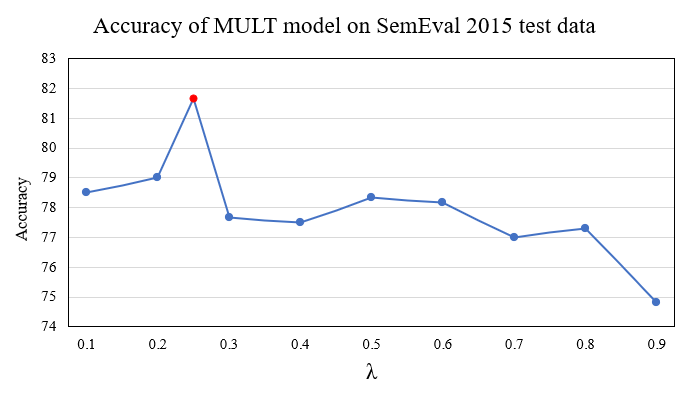
\includegraphics[scale=0.85]{Images/mult.PNG}
    \caption{Accuracy of the MULT model for different sizes of $\lambda$. The red data point is the optimal $\lambda$, at a value of 0.25.}
    \label{fig:multLambda}
\end{figure}



